\documentclass[hyperref={unicode}, 14pt]{beamer}

\sloppy

% Нумерация формул, таблиц и картинок относительно глав.
\EqInChapter
\TableInChapter
\PicInChapter

% Гипертекстовое оглавление.
\usepackage[
  bookmarks=true,  colorlinks=true, unicode=true,
  urlcolor=black,  linkcolor=black, anchorcolor=black,
  citecolor=black, menucolor=black, filecolor=black,
]{hyperref}

% Times, если стоит texlive-scalable-cyrfonts.
%\IfFileExists{cyrtimes.sty} {
  %\usepackage{cyrtimes}
%}

\usepackage{graphicx}
\graphicspath{{assets/}}

% Поля.
\geometry{right=15mm, top=20mm, bottom=20mm, left=30mm}

\usepackage{tikz}
\usetikzlibrary{arrows, arrows.meta}

\usepackage{pgfplots}
\pgfplotsset{compat=1.12}

\usepackage{enumerate}
\usepackage{multirow}
\usepackage{paralist, array}
\usepackage{fancyvrb}
\usepackage{changepage}

% Центрирование подписей.
\usepackage[justification=centering]{caption}

\newenvironment{conditions}[1][где]
  {#1 \begin{tabular}[t]{l @{~--- } l}}
  {\end{tabular}\\[\belowdisplayskip]}

\newenvironment{definition}[1]
  {\noindent#1\begin{adjustwidth}{.5\parindent}{}\noindent\ignorespaces}
  {\end{adjustwidth}}



\title{Полнотекстовой поиск}
\subtitle{в сети Интернет}
\author[Павелко П.Ю.]{Павелко П.Ю., ИУ7-61 \and Ломовской И.В., ИУ7}
\institute[]{МГТУ им. Баумана}
\date{Москва, \the\year}


\begin{document}

\begin{frame}
  \titlepage
\end{frame}

\begin{frame}
  \frametitle{Цели и задачи}

  \begin{block}{Цель}
    Разработка информационной системы для сбора информации в сети Интернет и последующего поиска по ней.
  \end{block}

  \begin{block}{Задачи}
    \begin{enumerate}
      \item Анализ предметной области;
      \item Разработка БД для хранения информации;
      \item Разработка поискового робота для сбора информации;
      \item Разработка программы для поиска;
      \item Разработка поисковой страницы;
    \end{enumerate}
  \end{block}
\end{frame}

\begin{frame}
  \frametitle{Полнотекстовой поиск}

  \begin{block}{Задача}
    Для заданного пользовательского запроса найти и отранжировать релевантные документы из выборки страниц сети Интернет.
  \end{block}

  \begin{block}{Этапы решения}
    \begin{itemize}
      \item Сбор информации
      \item Индексирование
      \item Поиск
    \end{itemize}
  \end{block}
\end{frame}

\begin{frame}
  \frametitle{IDEF0 поискового робота}

  \begin{center}
    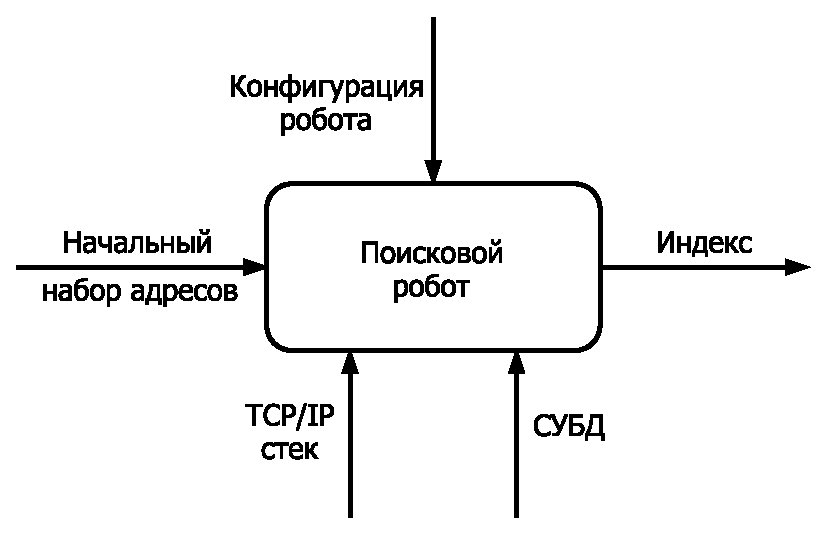
\includegraphics[width=\linewidth]{collecting-a0.pdf}
  \end{center}
\end{frame}

\begin{frame}
  \frametitle{IDEF0 поисковика}

  \begin{center}
    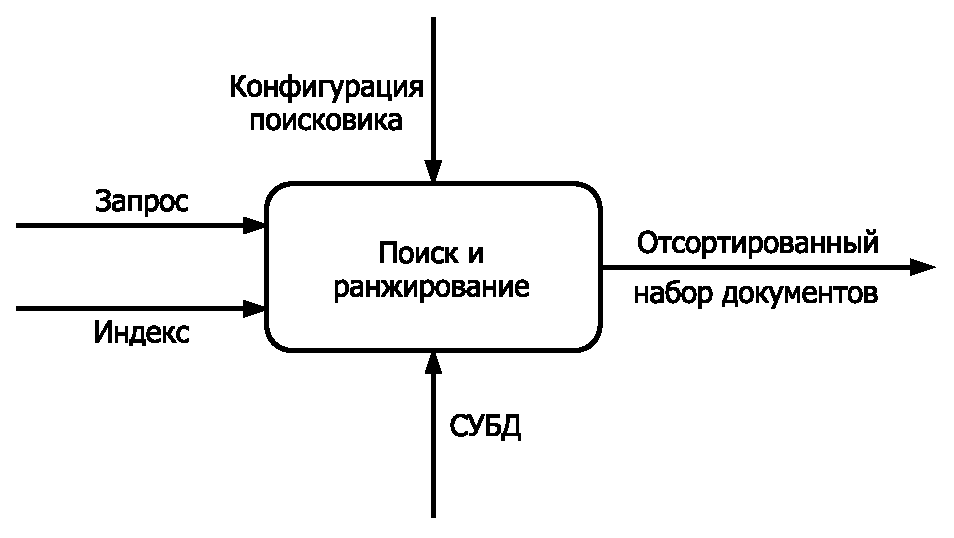
\includegraphics[width=\linewidth]{ranking-a0.pdf}
  \end{center}
\end{frame}

\begin{frame}
  \frametitle{ER-диаграмма предметной области}

  \begin{center}
    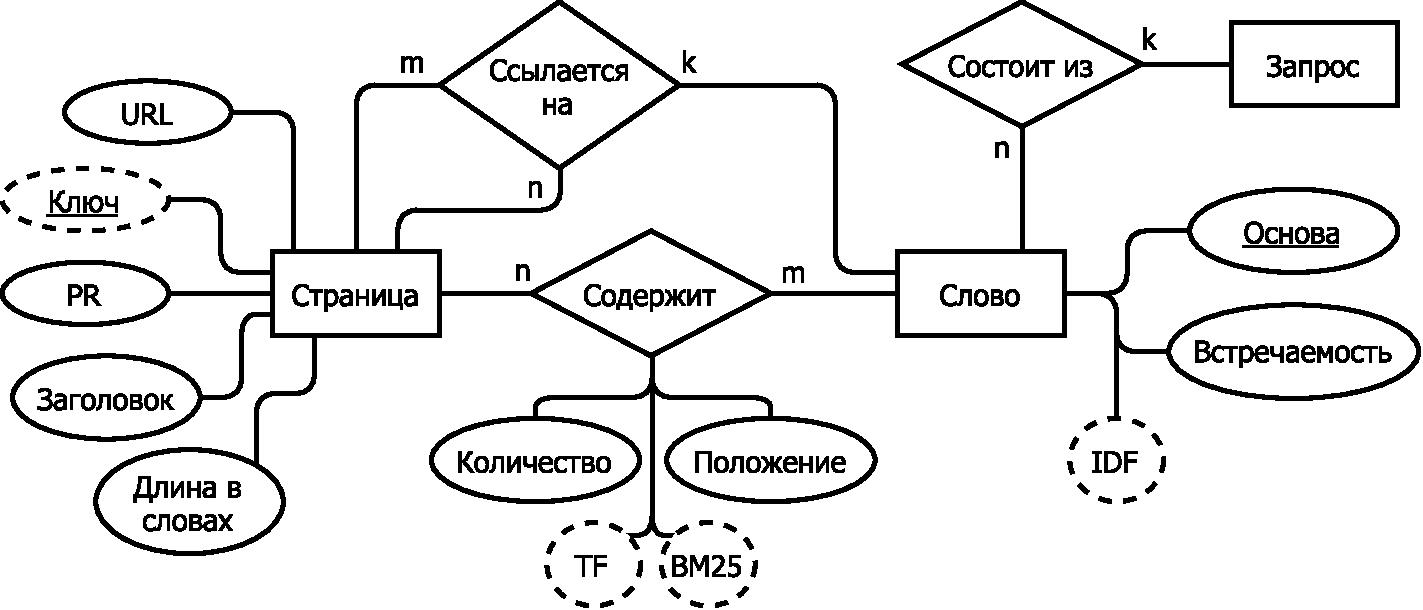
\includegraphics[width=\linewidth]{er.pdf}
  \end{center}
\end{frame}

\begin{frame}
  \frametitle{Архитектура поискового робота}

  \begin{center}
    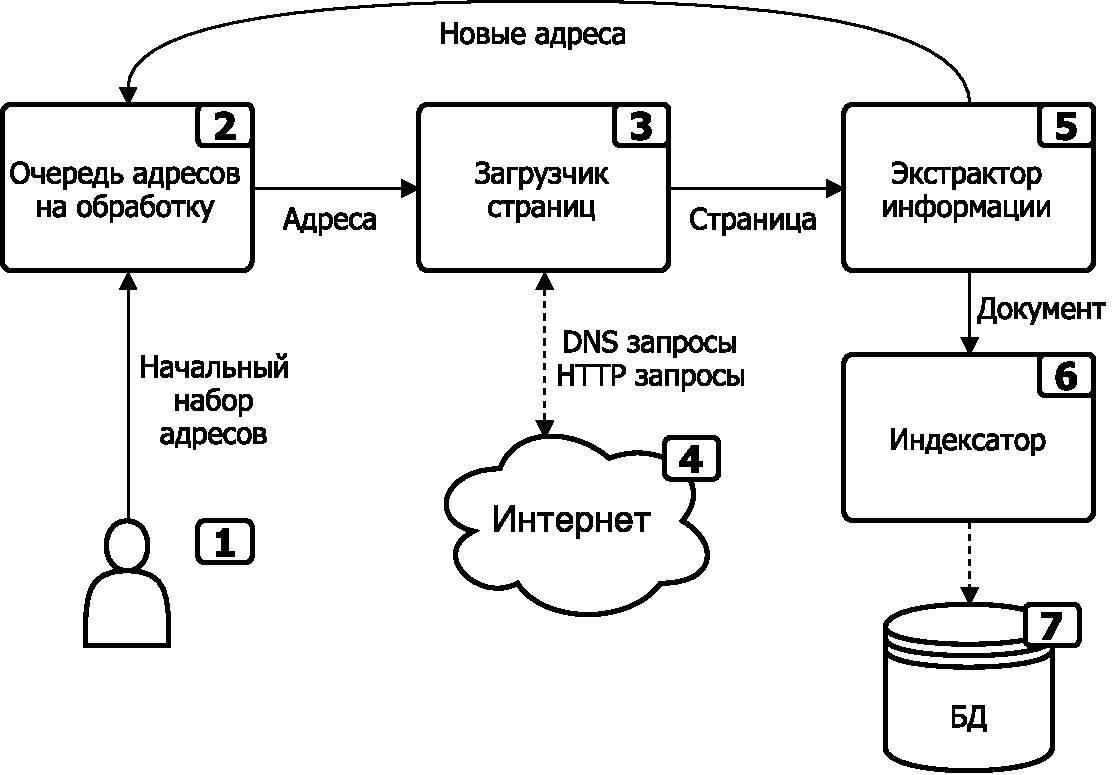
\includegraphics[height=.8\textheight]{crawler.pdf}
  \end{center}
\end{frame}

\begin{frame}
  \frametitle{База данных}

  \begin{center}
    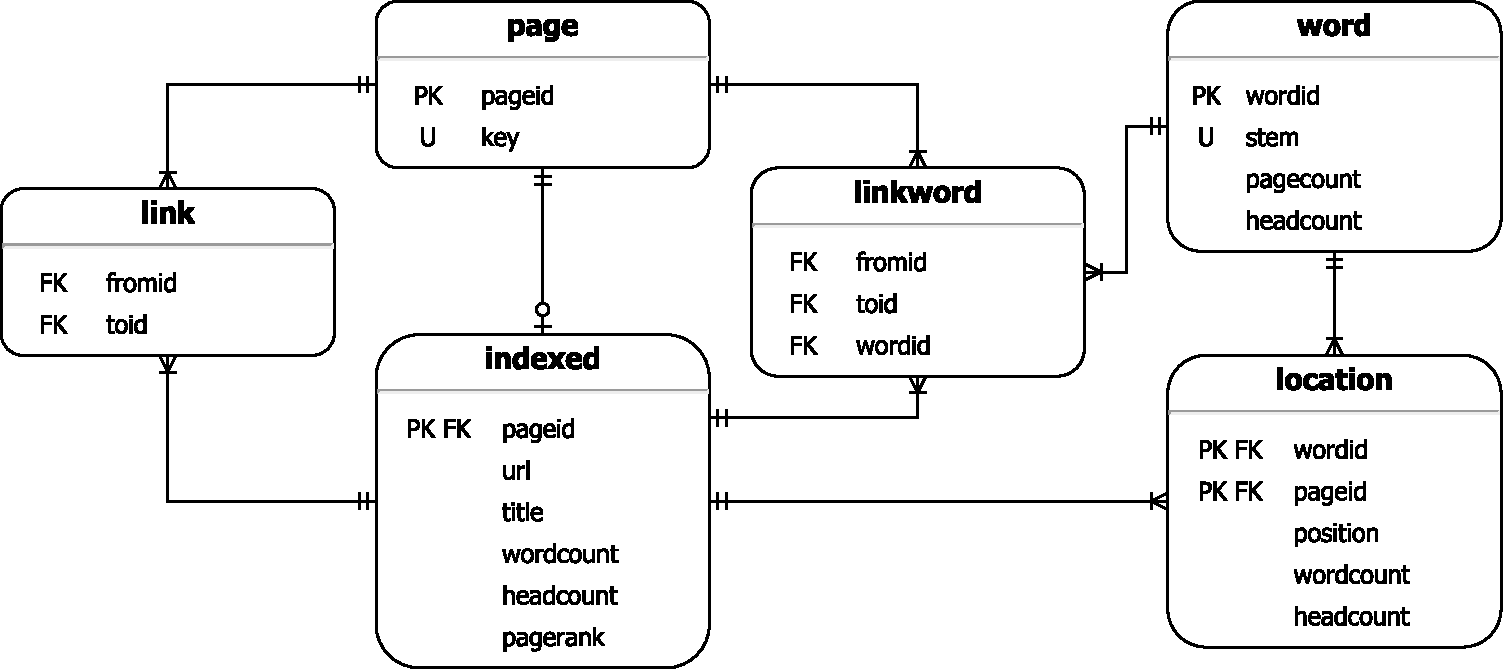
\includegraphics[width=\textwidth]{database.pdf}
  \end{center}
\end{frame}

\begin{frame}
  \frametitle{Поиск}

  \begin{block}{Этапы}
    \begin{enumerate}
      \item Извлечение из БД релевантных документов
      \item Подсчёт факторов
      \item Нормализация факторов
      \item Обработка выбросов
      \item Итоговое ранжирование
    \end{enumerate}
  \end{block}

  \begin{block}{Функция ранжирования}
    Итоговая функция ранжирования определяется как средневзвешенная сумма рассмотренных далее факторов.
  \end{block}
\end{frame}

\begin{frame}
  \frametitle{Ранжирование по содержимому}

  \begin{block}{}
    Данный класс факторов основывается на информации, которую можно получить непосредственно из документа.
  \end{block}

  \begin{block}{Факторы основываются на}
    \begin{itemize}
      \item Общем количестве слов в документе
      \item Частоте вхождения слов в документ
      \item Частоте вхождения слов в заголовки
      \item Положении запрошенных слов
      \item Расстоянии между запрошенными словами
    \end{itemize}
  \end{block}
\end{frame}

\begin{frame}
  \frametitle{Ссылочное ранжирование}

  \begin{block}{}
    \begin{enumerate}
      \item Использование текста ссылок
      \item PageRank
    \end{enumerate}
  \end{block}

  \begin{center}
    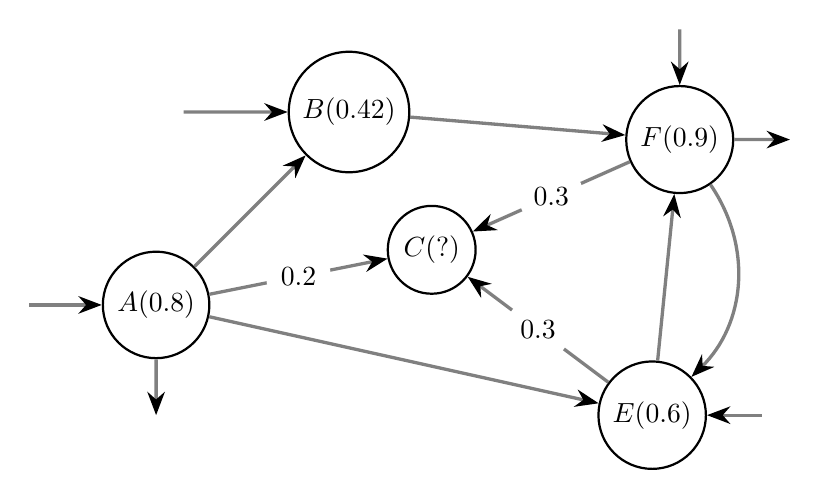
\begin{tikzpicture}[scale=.7]
      \begin{scope}[every node/.style={circle,thick,draw}]
        \node (A) at (-3.5,0) {$A (0.8)$};
        \node (B) at (0,3.5) {$B (0.42)$};
        \node (C) at (1.5,1) {$C (?)$};
        \node (E) at (5.5,-2) {$E (0.6)$};
        \node (F) at (6,3) {$F (0.9)$};
      \end{scope}

      \begin{scope}[>={Stealth[black]},
        every node/.style={fill=white,circle},
        every edge/.style={draw=gray,very thick}]
        \path[->] (A) edge node {$0.2$} (C);
        \path[->] (E) edge node {$0.3$} (C);
        \path[->] (F) edge node {$0.3$} (C);
        \path[->] (A) edge (B);
        \path[->] (A) edge (E);
        \path[->] (B) edge (F);
        \path[->] (E) edge (F);
        \path[->] (F) edge[bend left=40] (E);
        \path[<-] (E) edge ++(2,0);
        \path[->] (A) edge ++(0,-2);
        \path[<-] (A) edge ++(-2.3,0);
        \path[->] (F) edge ++(2,0);
        \path[<-] (F) edge ++(0,2);
        \path[<-] (B) edge ++(-3,0);
      \end{scope}
    \end{tikzpicture}
  \end{center}
\end{frame}

\begin{frame}
  \frametitle{Технологический слайд}

  \begin{block}{}
    \begin{itemize}
      \item Язык программирования: ECMAScript 2015 (JavaScript);
      \item Платформа: Node.js;
      \item Архитектура: событийно-ориентированная, асинхронная;
      \item СУБД: SQLite 3;
    \end{itemize}
  \end{block}
\end{frame}

\begin{frame}[plain]
  \centering
  {\Huge Спасибо за внимание!}\\[2cm]

  {\Large Московский государственный технический университет им Н.\,Э.~Баумана}\\[1cm]

  {\large Москва, \the\year}
\end{frame}

\end{document}

